\documentclass[12pt,oneside]{report}
%%%%%%%%%%%%%%%%%%%%%%%%%%%%%%%%%%%%%%%%%%%%%%%%%%%%%%%%%%%%%%%%%%%%%%%%%%%%%%%
\input{preambule_2020}
%%%%%%%%%%%%%%%%%%%%%%%%%%%%%%%%%%%%%%%%%%%%%%%%%%%%%%%%%%%%%%%%%%%%%%%%%%%%%%%
\portrait
%\paysage
%%%%%%%%%%%%%%%%%%%%%%%%%%%%%%%%%%%%%%%%%%%%%%%%%%%%%%%%%%%%%%%%%%%%%%%%%%%%%%%

%À modifier !!!!!!!!!!!!!!!!!!!!!!!!!!!!!!!!
\newcommand{\classe}{Remise à niveau}
\newcommand{\anneescol}{Année 2020-2021}
\newcommand{\numdm}{3}
\newcommand{\numds}{3}

%entête DM

\fancypagestyle{garde_dm}{% 
%\fancyhead[C]{\small\textbf{Nom,  Prénom : }\makebox[5cm]{\dotfill}\hfill \small \textbf{\tesspe - 2016/2017}}
\renewcommand{\headrulewidth}{0cm}}


\newcommand{\tete}{
\thispagestyle{garde_dm}

\begin{center}
\begin{CadreModule}{}
\vspace*{1em}
\begin{tabular}{m{0.15\linewidth}M{0.63\linewidth}R{0.15\linewidth}}
\includegraphics[width=\linewidth]{logo_augustin_thierry}
&
%\textbf{\large DEVOIR MAISON DE MATH\'EMATIQUES N\degres \numdm}\par\medskip
{\fontfamily{pzc}
\bfseries\fontsize{20}{20}\selectfont{Tableaux de signes}}
&
\includegraphics[width=\linewidth]{logo_augustin_thierry}
\end{tabular}
\vspace*{0.2em}
\end{CadreModule}
\end{center}

%\begin{CadreModule}{}
%\begin{center}
%Le travail et le rendu en groupe est autorisé.
%
%L'exercice \og niveau 1 \fg{}  est \textbf{obligatoire}.
%L'exercice \og niveau 2 \fg{} est \textbf{conseillé}.
%
%L'exercice \og niveau 3 \fg{} est \textbf{facultatif}.
%\end{center}
%\end{CadreModule}

\noindent
\vspace{-1.5em}
}

%%%%%%%%%%%%%%%%%%%%%%%%%%%%%%%%%%%%%%%%%%%%%%%%%%%%%%%%%%%%%%%%%%%%%%%%%%%%%%%
%%%%%%%%%%%%%%%%%%%%%%%%%%%%%%%%%%%%%%%%%%%%%%%%%%%%%%%%%%%%%%%%%%%%%%%%%%%%%%%
%\tikzset{domaine/.style 2 args={domain=#1:#2}}
%%%%%%%%%%%%%%%%%%%%%%%%%%%%%%%%%%%%%%%%%%%%%%%%%%%%%%%%%%%%%%%%%%%%%%%%%%%%%%%
%%%%%%%%%%%%%%%%%%%%%%%%%%%%%%%%%%%%%%%%%%%%%%%%%%%%%%%%%%%%%%%%%%%%%%%%%%%%%%%

%%%%%%%%%%%%%%%%%%%%%%%
%% DEBUT DU DOCUMENT %%
%%%%%%%%%%%%%%%%%%%%%%%

\begin{document}
%\selectlanguage{english}
\selectlanguage{french}
\setlength\parindent{0mm}
\tete 		%entête classique

\renewcommand \footrulewidth{0.2pt}%
\renewcommand \headrulewidth{0pt}%
\pagestyle{fancy}
\fancyhf{}
\pieddepage{\classe}{\thepage / \pageref{LastPage}}{\anneescol}

%%%%%%%%%%%%%%%%%%%%%%%%%%%%%%%%%%%%%%%%%%%%%%%%%%%%%%%%%%%%
\begin{spacing}{1.2}
%%%%%%%%%%%%%%%%%%%%%%%%%%%%%%%%%%%%%%%%%%%%%%%%%%%%%%%%%%%%

\begin{center}
\begin{tikzpicture}
\tkzTabInit[color,lgt=2,espcl=3,colorC=blue!20,colorV=blue!20]
{$x$ / 1 ,Signe\\de $A(x)$ / 1.5}
{$-\infty$, $\frac{7}{8}$, $+\infty$}
\tkzTabLine{,-,z,+,}
\end{tikzpicture}
\end{center}

\begin{center}
\begin{tikzpicture}
\tkzTabInit[color,lgt=2,espcl=3,colorC=blue!20,colorV=blue!20]
{$x$ / 1 ,Signe\\de $B(x)$ / 1.5}
{$-\infty$, $\frac{5}{2}$, $+\infty$}
\tkzTabLine{,+,z,-,}
\end{tikzpicture}
\end{center}

\begin{center}
\begin{tikzpicture}
\tkzTabInit[color,lgt=2,espcl=2,colorC=blue!20,colorV=blue!20]
{$x$/1,$\frac{1}{3}-\frac{5}{2}x$/1,$7-\frac{1}{2}x$/1 ,Signe\\de $C(x)$ / 1.5}
{$-\infty$, $\frac{2}{15}$,$14$, $+\infty$}
\tkzTabLine{,+,z,-,t,-,}
\tkzTabLine{,+,t,+,z,-,}
\tkzTabLine{,+,z,-,z,+,}
\end{tikzpicture}
\end{center}

\begin{center}
\begin{tikzpicture}
\tkzTabInit[color,lgt=2,espcl=2,colorC=blue!20,colorV=blue!20]
{$x$/1,$x$/1,$9x+1$/1 ,Signe\\de $D(x)$ / 1.5}
{$-\infty$, $\frac{-1}{9}$,$0$, $+\infty$}
\tkzTabLine{,-,t,-,z,+,}
\tkzTabLine{,-,z,+,t,-,}
\tkzTabLine{,+,d,-,z,+,}
\end{tikzpicture}
\end{center}

%%%%%%%%%%%%%%%%%%%%%%%%%%%%%%%%%%%%%%%%%%%%%%%%%%%%%%%%%%%%
\end{spacing}
%%%%%%%%%%%%%%%%%%%%%%%%%%%%%%%%%%%%%%%%%%%%%%%%%%%%%%%%%%%%
%%%%%%%%%%%%%%%%%%%%%
%% FIN DU DOCUMENT %%
%%%%%%%%%%%%%%%%%%%%%
\end{document}